\documentclass[10pt]{article}
\usepackage{fullpage}
\usepackage{graphicx}
\usepackage{amsmath}

\author{Tom Selier}
\title{Deriving equations of motions of a cart pendulum using the Lagrangian}
\date{\today}
\graphicspath{
    {img/}
}

\begin{document}

    \maketitle

    \section{Introduction}
    This is the introduction.

    \section{The system}
    \begin{figure}{t}
        \centering
        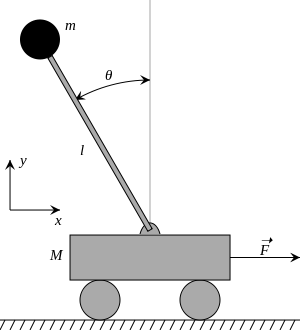
\includegraphics[width=4cm]{Cart-pendulum.png}
        \caption{The pendulum}
        \label{fig:system}
    \end{figure}
    
    Where in figure \ref{fig:system}: \\
    \qquad $m$: Mass of the pendulum  [kg] \\
    \qquad $M$: Mass of the cart  [kg] \\
    $\theta$: Degrees pendulum in reference to the cart [rad] \\
    $\ell$: Length of the pendulum [m] \\
    $x$: Position of the cart [m]

    \section{Lagrangian}
    Let the position and velocity of the pendulum be
    \begin{align*}
        x_s &= x + \ell  sin(\theta) \\
        y_s &= - \ell  cos(\theta) \\
        \dot x_s &= \dot x + \ell  \dot \theta  cos(\theta) \\
        \dot y_s &= \ell  \dot \theta  sin(\theta)
    \end{align*}

    Then, to derive the equations of motion, the Lagrangion will be used.
    First, $T$, the kinetic energy of the system will be calculated.

    \begin{equation}
        \begin{aligned}
            T &= \frac{1}{2}  M  \dot x^2 + \frac{1}{2}  m (\dot x_s^2 + \dot y_s^2) \\
            T &= \frac{1}{2}  M  \dot x^2 + \frac{1}{2} m((\dot x + \ell  \dot \theta  cos(\theta))^2 + (\ell  \dot \theta  sin(\theta))^2) \\
            T &= \frac{1}{2}  M  \dot x^2 + \frac{1}{2}  m(\dot x^2 + 2 \dot x  \ell  \dot \theta  cos(\theta) + \ell^2  \dot \theta^2 cos(\theta)^2 + \ell^2  \dot \theta^2  sin(\theta)^2) \\
            T &= \frac{1}{2}  M  \dot x^2 + \frac{1}{2} m(\dot x^2 + 2 \dot x \ell \dot \theta cos(\theta) + \ell^2 \dot \theta^2) \\
            T &= \frac{1}{2}(M + m) \dot x^2 + \frac{1}{2}m(2 \dot x \ell \dot \theta cos(\theta) + \ell^2 \dot \theta^2) \\
            T &= \frac{1}{2}(M + m) \dot x^2 + m \dot x \ell \dot \theta cos(\theta) + \frac{1}{2}m \ell^2 \dot \theta^2 
        \end{aligned}
    \end{equation}

    
\end{document}